As in previous sprint chapters, work-flow trough sprint 5 will be described. What makes this sprint different from the others, is that the team had to manage occurred risk on communication module. A good part of this chapter will be devoted to resolution of risk, but it will not lack the rest of the processes such as planning, establishing goals and retrospective.


\section{Sprint planning}

The planning started with customer meeting at Thursday 24th of October 2013. For customer, main event and goal of this sprint is finalizing prototype and recording demo video. Therefore planning includes tasks as: collecting phones from friends, researching the companies that do mobile development and borrowing the phones from them, renting the room and recording equipment from university.

Team agreed that borrowing phones from companies should be backup plan since sufficient number of phones (at least 16) can be collected from friends and colleagues. 

Recording final demo is planned for Thursday 7th of November, and informing potential phone owners that will be able to share their phones with us is planned at least one week before the event. This way table of potential phones can be crated, and risk of not collecting the sufficient number of devices can be reduced and solved. 

Recording equipment is planned to be rented or reserved at least 3 days before the event. 

\subsection{User-stories}
\subsubsection*{Implementation}
All the functional requirements for sprint 5 are presented in table \ref{tab:sprint5stories}
\LTXtable{\textwidth}{sprint5/stories.tex}

\subsubsection*{Documentation}
All the documentation stories for sprint 5 are presented in table \ref{tab:sprint5Documentationstories}
\LTXtable{\textwidth}{sprint5/storiesDocumentation.tex}

\subsubsection*{Project management}
All the project management for sprint 5 are presented in table \ref{tab:sprint5storiesProcess}
\LTXtable{\textwidth}{sprint5/storiesProcess.tex}

% hous all in total: Estimated: 235  Spent: 230


\section{Sprint Goal}

On the end of this sprint team expect to have working, the prove of concept demo. As core modules are finished, team will invest time in tuning existing and implementing some of the supporting functionalities. Some of them are: speeding up the detection process  and preparing predefined gallery to be played. Goal for this sprint is also a time sync between server and clients. Reason is bypassing possible networking latency, and enabling clients to play the content more precise. 

\section{Duration}
This sprint is 2 weeks long. From 28th of October 2013 to 10th of November 2013. 
Team agreed on the date of presentation and showing the running demo – on Thursday 7th of November 2013.
Estimated velocity is 200 hours since every team member will devote 25 working hours per week.

\section{Architecture}

At first team was thinking about implementing the clock synchronization from scratch. Using one of the popular algorithms as Berkeley algorithm\footnote{http://ieeexplore.ieee.org/stamp/stamp.jsp?tp=\&arnumber=29484}, and adding additional responsibility to server or client application. 

The Barkley algorithm requires feedback communication from clients by implementing receiving message system on server. Calculating the time offset on server and adjusting local times on clients. The protocol will have to expended in order to support clock sync communication. Although this approach will work, lot of changes on existing architecture have to be done.

As focus of this project is on proving the concept, and customer want all hours devoted on project to be spent well, team was agreed on researching alternative solutions before start implementing. Further research have brought to Network Time Protocol(NTP)\footnote{https://tools.ietf.org/html/rfc5905\#section-14}.

Good thing about NTP is that NTP is used for variable-latency data networks. It was only needed to find application that provide NTP service, and change client code to call this service and determine what is a local time offset before connecting to Digital Lighter server application. In that case, change of existing architecture will be minimal, and it will play only on client application. No server, or protocol will have to be changed.

As solution Time Server\footnote{https://play.google.com/store/apps/details?id=com.icecoldapps.timeserver} application have been chosen. It will work on same device as Digital Lighter server application, and it will provide same time as Digital Lighter application would. Deployment digram is therefore changed, and now includes NTP server as artifact. 

\begin{figure}[H]
	\centering
		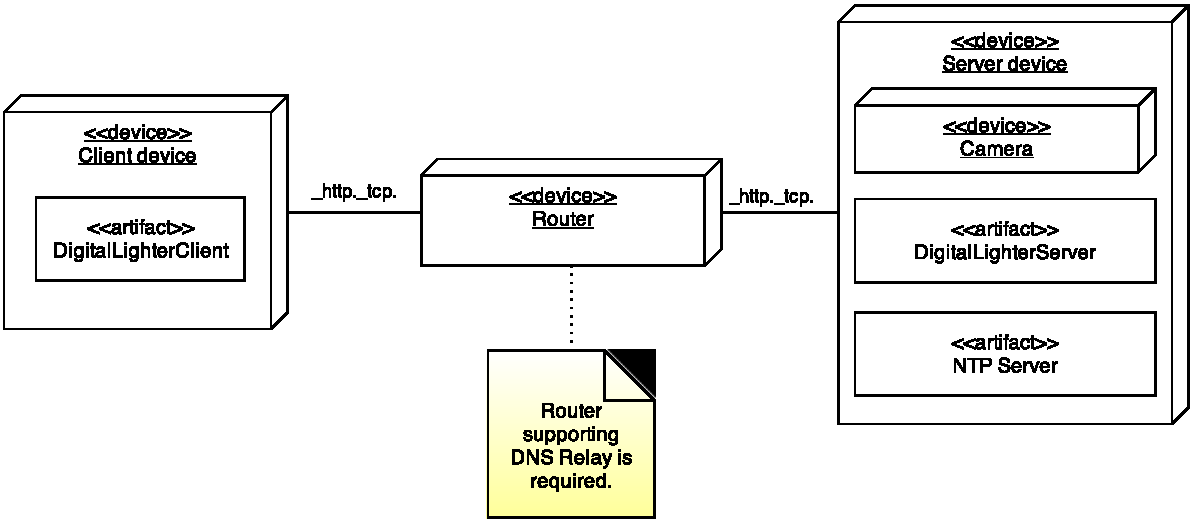
\includegraphics[width=15cm]{images/deployment-diagram-sprint5}
	\caption{Deployment diagram}
	\label{fig:sprint5_deployment_diagram}
\end{figure}

Change have influence on messages interchange between server and clients. The difference comparing to old sequence diagram is given at Figure \ref{fig:sprint5_sequence_diagram}. New calls are colored with red color. 

\begin{figure}[H]
	\centering
		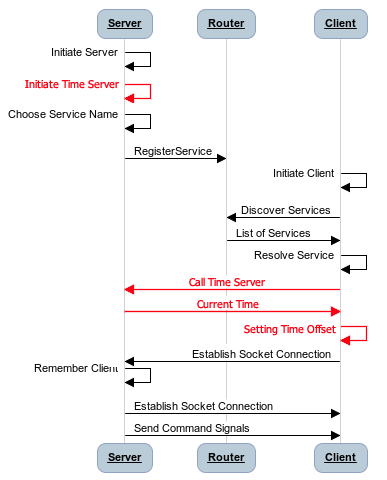
\includegraphics[width=9cm]{sprint5/communication}
	\caption{Sequence diagram}
	\label{fig:sprint5_sequence_diagram}
\end{figure}

Observing deployment and sequence diagrams, it is easy to see that this solution didn't need existing system to change. But in same time new functionality have been added. This way project architecture follows open/closed principle\footnote{http://msdn.microsoft.com/en-us/magazine/cc546578.aspx}. System is closed for changes, but open for extensions.

\section{Implementation}

\begin{figure}[H]
	\centering
		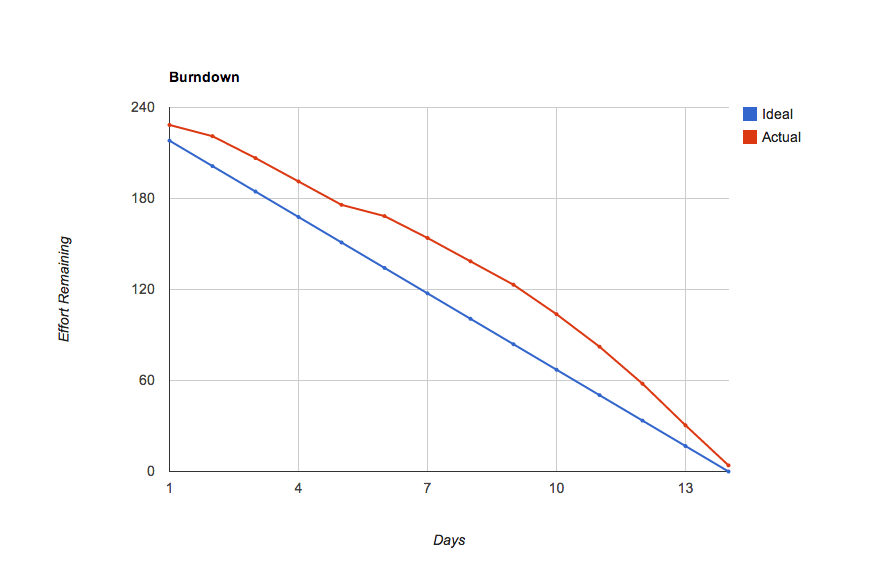
\includegraphics[width=18cm]{sprint5/BurndownSprint5.png}
	\caption{Burn down chart.}
	\label{fig:Burn5 }
\end{figure}



\section{Testing}
\section{Occurring risks}
\section{Customer feedback}
\section{Retrospective}
This section reflects on the past sprint. In order to learn from the mistakes done and thus to improve the workflow it is necessary to answer two essential questions: "What went well" and "What could be improved".

\subsection{What went well}
\subsection{What could be improved}
